
\section{Objective}

\begin{enumerate}[label=(\roman*)]
    \item To study the input and output characteristics of a PNP transistor in Common Base mode and determine transistor parameters.
    \item To study the input and output characteristics of an NPN transistor in Common Emitter mode and determine transistor parameters.
\end{enumerate}

\section{Theory}

A Bipolar Junction Transistor, or BJT is a three terminal device having two PN-junctions connected together in series. Each terminal is given a name to identify it and these are known as the Emitter (E), Base (B) and Collector (C). There are two basic types of bipolar transistor
construction, NPN and PNP, which basically describes the physical arrangement of the P-type and N-type semiconductor materials from which they are made. 

Bipolar Transistors are \textit{current amplifying} or current regulating devices that control the amount of current flowing through them in proportion to the amount of biasing current applied to their base terminal. The principle of operation of the two transistor types NPN and PNP, is exactly the same the only difference being in the biasing (base current) and the polarity of the power supply for each type.

\begin{figure}[H]
    \centering
    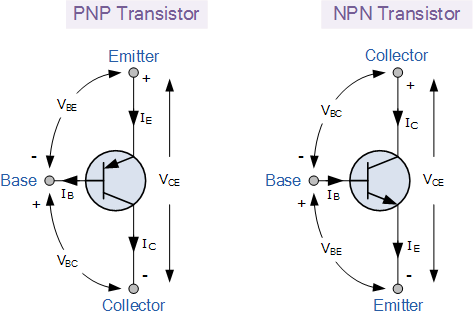
\includegraphics[width=.9\columnwidth]{images/f1.jpg}
    \caption{Schematic diagram and conventional current flows in NPN and PNP transistors}
        \label{fig:3}
\end{figure}

The symbols for both the NPN and PNP bipolar transistor are shown above along with the direction of conventional current flow. The direction of the arrow in the symbol shows current flow between the base and emitter terminal, pointing from the positive P-type region to the negative N-type region, exactly the same as for the standard diode symbol. For normal operation, the emitter-base junction is forward-biased and the collector-base junction is reverse-biased.

\subsection*{Transistor Configurations}

There are three possible configurations possible when a transistor is connected in a circuit: (a) Common base, (b) Common emitter (c) Common collector. We will be focusing on the first two configurations in this experiment. 

The behaviour of a transistor can be represented by d.c. current-voltage (I-V) curves, called the static characteristic curves of the device. The three important characteristics of a transistor are: (i) Input characteristics, (ii) Output characteristics and (iii) Transfer Characteristics. These characteristics give information about various transistor parameters, e.g. input and out dynamic resistance, current amplification factors, etc.

\subsection{Common Base Transistor Characteristics}

In common base configuration, the base is made common to both input and output as shown in its circuit diagram.\\

\begin{enumerate}
\item \textbf{Input Characteristics:}
    The input characteristics is obtained by plotting a curve between $I_E$ and $V_{EB}$ keeping voltage $V_{CB}$ constant. This is very similar to that of a forward-biased diode and the slope of the plot at a given operating point gives information about its input dynamic resistance.\\

    \textbf{Input Dynamic Resistance} ($r_i$) is defined as the ratio of change in base emitter voltage ($\Delta V_{EB}$) to the resulting change in emitter current ($\Delta I_E$) at constant collector-emitter voltage ($V_{CB}$). This is dynamic as its value varies with the operating current in the transistor.
    \begin{align}
        r_i = \frac{\Delta V_{EB}}{\Delta I_E}\Bigm|_{V_{CB}}
    \end{align}\\

\item \textbf{Output Characteristics:}
    The output characteristic curves are plotted between $I_C$ and $V_{CB}$, keeping $I_E$ constant. The output characteristics are controlled by the input characteristics. Since $I_C$ changes with $I_E$, there will be different output characteristics corresponding to different values of $I_E$. These curves are almost horizontal. This shows that the output dynamic resistance, defined below, is very high.\\

    \textbf{Output Dynamic Resistance} ($r_o$) is defined as the ratio of change in collector-base voltage ($\Delta V_{CB}$) to the change in collector current ($\Delta I_C$) at a constant base current $I_E$.
    \begin{align}
        r_o = \frac{\Delta V_{CB}}{\Delta I_C}\Bigm|_{I_E}
    \end{align}\\

\item \textbf{Transfer Characteristics:}
    The transfer characteristics are plotted between the input and output currents ($I_E$ versus $I_C$).\\

    \textbf{Current amplification factor} ($\alpha$) is defined as the ratio of the change in collector current to the change in emitter current at a constant collector-base voltage ($V_{CB}$) when the transistor is in active state.
    \begin{align}
        \alpha_{ac} = \frac{\Delta I_C}{\Delta I_E}\Bigm|_{V_{CB}}
    \end{align}
    This is also known as small signal current gain and its value is very large. The ratio of $I_C$ and $I_E$ is called $\alpha_{dc}$ of the transistor. Hence,
    \begin{align}
        \alpha_{dc} = \frac{I_C}{I_E}\Bigm|_{V_{CB}}
    \end{align}
    Since $I_C$ increases with $I_E$ almost linearly, the values of both $\alpha_{dc}$ and $\alpha_{ac}$ are nearly equal.

\end{enumerate}

\subsection{Common Emitter Transistor Characteristics}

In common emitter configuration, the emitter is made common to both input and output as shown in its circuit diagram.\\

\begin{enumerate}

\item \textbf{Input Characteristics:}
    The variation of the base current $I_B$ with the base-emitter voltage $V_{BE}$ keeping the collector-emitter voltage $V_{CE}$ fixed, gives the input characteristic in CE mode.\\

    \textbf{Input Dynamic Resistance} ($r_i$) is defined as the ratio of change in base emitter voltage ($\Delta V_{BE}$) to the resulting change in base current ($\Delta I_B$) at constant collector-emitter voltage ($V_{CE}$). This is dynamic as its value varies with the operating current in the transistor.
    \begin{align}
        r_i = \frac{\Delta V_{BE}}{\Delta I_B}\Bigm|_{V_{CE}}
    \end{align}\\

\item \textbf{Output Characteristics:}
    The variation of the collector current $I_C$ with the collector-emitter voltage $V_{CE}$ is called the output characteristic. The plot of $I_C$ versus $V_{CE}$ for different fixed values of $I_B$ gives one output characteristic. Since the collector current changes with the base current, there will be different output characteristics corresponding to different values of $I_B$.\\

    \textbf{Output Dynamic Resistance} ($r_o$) is defined as the ratio of change in collector-emitter voltage ($\Delta V_{CE}$) to the change in collector current ($\Delta I_C$) at a constant base current $I_B$.
    \begin{align}
        r_o = \frac{\Delta V_{CE}}{\Delta I_C}\Bigm|_{I_B}
    \end{align}\\

\item \textbf{Transfer Characteristics:} 
    The transfer characteristics are plotted between the input and output currents ($I_B$ versus $I_C$), which increase proportionately.\\

    \textbf{Current amplification factor} ($\beta$) is defined as the ratio of the change in collector current to the change in base current at a constant collector-emitter voltage ($V_{CE}$) when the transistor is in active state.
    \begin{align}
        \beta_{ac} = \frac{\Delta I_C}{\Delta I_B}\Bigm|_{V_{CE}}
    \end{align}
    This is also known as small signal current gain and its value is very large. The ratio of $I_C$ and $I_B$ is called $\beta_{dc}$ of the transistor. Hence,
    \begin{align}
        \beta_{dc} = \frac{I_C}{I_B}\Bigm|_{V_{CE}}
    \end{align}
    Since $I_C$ increases with $I_B$ almost linearly, the values of both $\beta_{dc}$ and $\beta_{ac}$ are nearly equal.

\end{enumerate}

\subsection*{Applications}

Transistors are used in everyday life in many forms, like amplifiers and switching apparatuses. As amplifiers, they are being used in various oscillators, modulators, detectors and nearly any circuit to perform a function. In a digital circuit, transistors are used as switches.